
\documentclass[12pt]{beamer}

\usepackage[white]{beamerthemeWisconsin}
\usepackage{framed}
\usepackage{tikz}
%\usetheme[white]{Wisconsin}
\graphicspath{{./}{./uw-beamer-template/}{../images/}}
\title{Leveraging Intel's Embree Ray Tracing in the DAGMC Toolkit}
\author{Patrick C Shriwise}
\institute{University of Wisconsin - Madison}
\date{ANS Winter Meeting 2015}




\AtBeginSection[]{
  \begin{frame}
  \vfill
  \centering
  \begin{beamercolorbox}[sep=8pt,center,shadow=true,rounded=true]{title}
    \usebeamerfont{title}\insertsectionhead\par%
  \end{beamercolorbox}
  \vfill
  \end{frame}
}


%%%% TIKZ OBJECTS %%%%
\usetikzlibrary{shapes}
\usetikzlibrary{positioning}
\usetikzlibrary{decorations.pathreplacing}

\tikzset{every node/.style={inner sep=0pt, outer sep=1pt}}
\tikzstyle{uwstep} = [minimum width=2.5cm, minimum height=1cm,text centered, text width=2.5cm, draw=black, fill=UWRed, text=white]

\tikzstyle{embreestep} = [ellipse, minimum width=2.5cm, minimum height=1cm,text centered, text width=2cm, draw=black, fill=blue, text=white]

\tikzstyle{arrow} = [thick,->,>=stealth]

\tikzset{
    myarrow/.style={
        draw,
        fill=UWRed,
        single arrow,
        minimum height=4ex,
        single arrow head extend=1ex
    }
}

\newcommand{\arrowup}{%
\tikz [baseline=-0.5ex]{\node [myarrow,rotate=90] {};}
}
\newcommand{\arrowdown}{%
\tikz [baseline=-1ex]{\node [myarrow,rotate=-90] {};}
}
\newcommand{\arrowright}{%
\tikz [baseline=-0.5ex]{\node [myarrow,rotate=0] {};}
}
\newcommand{\doublearrow}{%
\tikz [baseline=-1ex]{\node [mydoublearrow,rotate=0] {};}
}



%%%% START DOCUMENT %%%%
\begin{document}


%% Title Frame %%
\frame{\titlepage \addtocounter{framenumber}{-1}}


%%Outline%%
\begin{frame}
\frametitle{\null}
\tableofcontents
\end{frame}

%% Introduction %%
\section{CAD-Based Monte Carlo Transport} % 1-2 slides
% We use it for our geometric queries:
   % point-inclusion
   % dist to next surf
% Replaces analytic intersections in native MonteCarlo packages
% Motivation: takes too long!
% Images of typical production models?
\begin{frame}

\frametitle{Robust CAD-Based Monte Carlo Transport}

DAGMC can robustly do transport calculations on highly detailed CAD models like these:


\begin{center}
\begin{tabular}{c c}

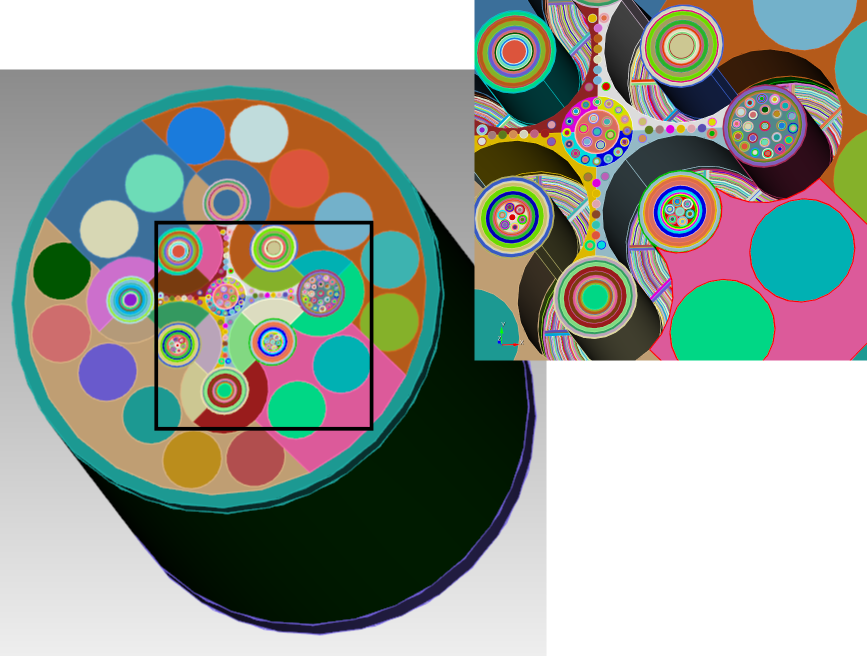
\includegraphics[height=0.4\textheight]{atr_both.png} &
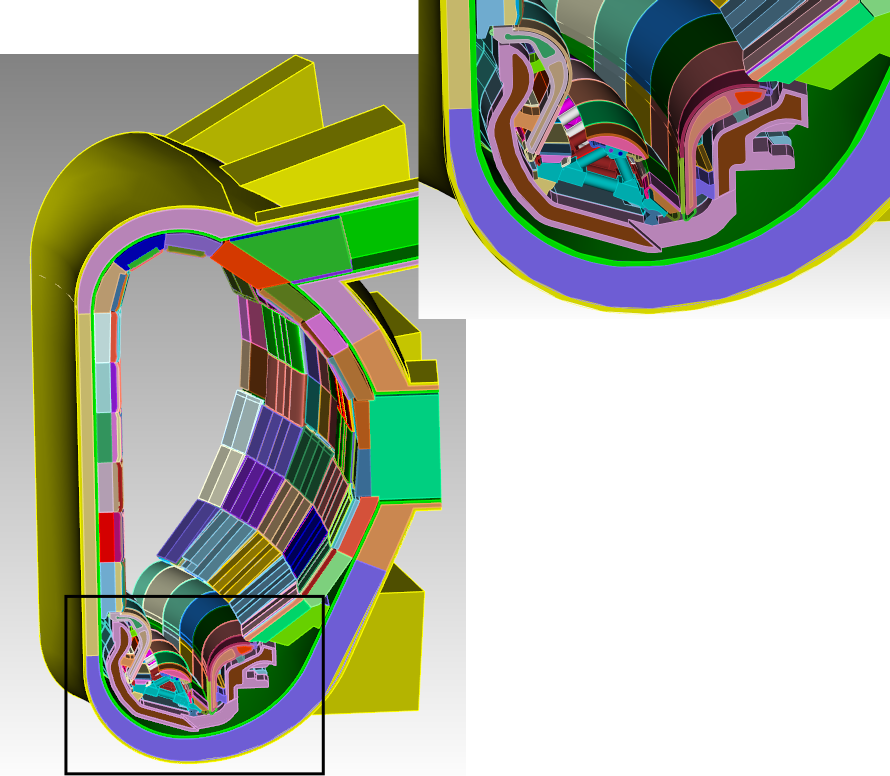
\includegraphics[height=0.4\textheight]{bllite_both.png} \\

\small Advanced Test Reactor &
\small ITER \\

\end{tabular}
\end{center}

But it takes a long time... (2-10x slower than native codes)

\end{frame}

%% \begin{frame}
%% \frametitle{DAGMC Workflow}
%% \begin{center}
%% \begin{tikzpicture}
%%   \node (CAD) [uwstep] {\small CAD \\ Geometry};

%%   \node (CUBIT) [uwstep, xshift=3cm, label=below:{\small imprint \& merge}] {\small CUBIT};
  
%%   \node (PREPROC) [uwstep, xshift=6cm, label=below:{\small surface faceting}] {\small dagmc \\preproc};

%%   \node (MW) [uwstep, xshift=9cm, label={\small facet sealing}] {\small make \\watertight};

%%   \node (MC) [uwstep, xshift=9cm, yshift=-2cm, label=below:{\small analysis}] {\small Monte Carlo};

%%   \draw [arrow] (CAD) -- (CUBIT);

%%   \draw [arrow] (CUBIT) -- (PREPROC);

%%   \draw [arrow] (PREPROC) -- (MW);

%%   \draw [arrow] (MW) -- (MC);

%% \end{tikzpicture}
%% \end{center}

%% \end{frame}

\begin{frame}

  \frametitle{DAGMC \& Ray Tracing}
  
  The typical statment is that we save much of our human time typically spent defining the model using outdated geometry systems at the expense of this extra computing time. \\

  A great deal of human time is saved in dealing with outdated geometric representations at the cost of extra computing time
 \vfill
 
 What if we could drastically reduce this extra computing time?

 \vfill

  
\end{frame}

\begin{frame}

\frametitle{Ray Tracing in DAGMC}
\vfill
 85\% of the time spent in DAGMC runs is in the ray tracing of the discretized (faceted) model.
\vfill 
\begin{itemize}
\item point-inclusion tests
\item next surface distance determination
\end{itemize}



\end{frame}

\section{Ray Tracing Accelerations} % 2-3 slides
% BVH explanation in 1 slide
% Embree's tricks
% Extra: SAH


\begin{frame}
\frametitle{Bounding Volume Hierarchies}


By partitioning the geometry-based meshes using bounding volumes, we gain significant improvements over a linear search of the discrete elements.
\begin{columns}
  \column{0.5\textwidth}
  \begin{figure}
    \centering
    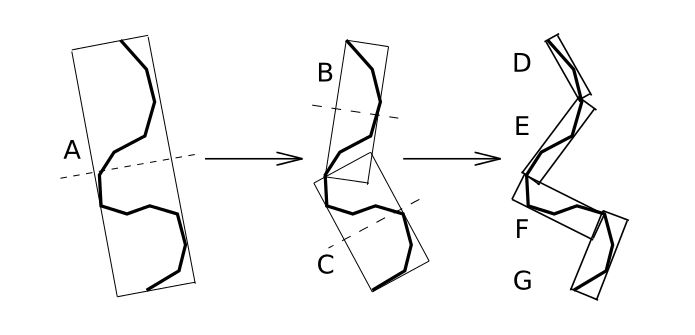
\includegraphics[width=1.1\textwidth]{bvh_2d_ex_w_labels.png} 
    \cite{gottschalk1996obbtree}
  \end{figure}
  
  \column{0.4\textwidth}
  \begin{figure}
    \centering
    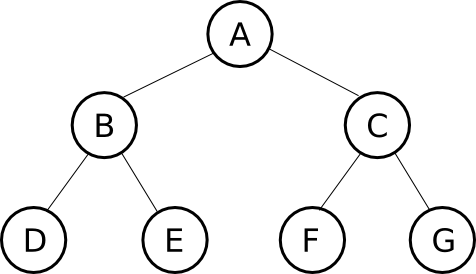
\includegraphics[width=0.5\textwidth]{binary_graph.png}
  \end{figure}
\end{columns}

How we create these bounding volume hierarchies (BVHs) matters \textbf{a lot} in terms of the performance.


\end{frame}

\begin{frame}
\frametitle{DAGMC's BVH}

DAGMC uses the BVH hierarchy found in the Mesh Oriented dAtaBase, MOAB.
\begin{center}
  \begin{tikzpicture}

    \node (SHALLOW) [auto, outer sep=10pt, label=below:{\small shallow}] {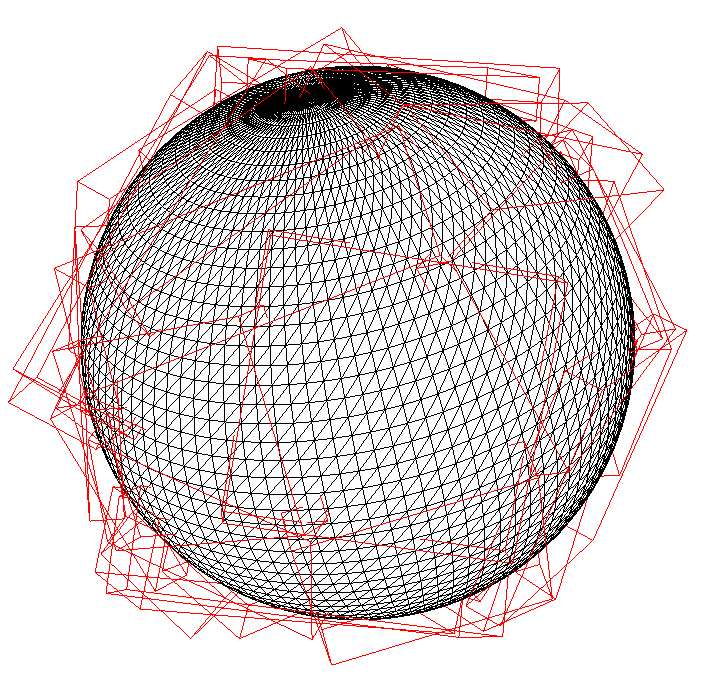
\includegraphics[width=0.3\textwidth]{sphere_obbs_shallow.png}};
    \node [myarrow,rotate=0,xshift=3.5cm] {};
    \node (DEEP) [auto, outer sep=10pt, xshift=7cm, label=below:{\small deep}] {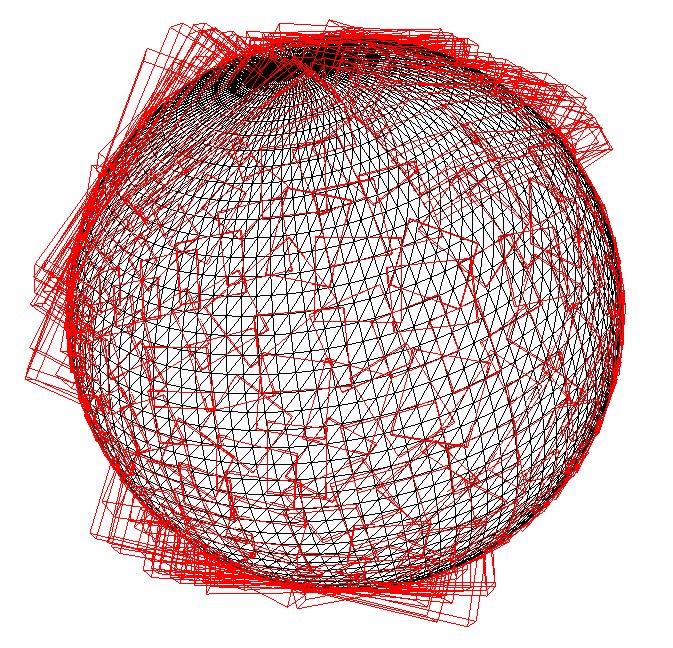
\includegraphics[width=0.3\textwidth]{sphere_obbs_deep.png}};

   % \draw [arrow] (SHALLOW) -- (DEEP);
  \end{tikzpicture}
\end{center}

\begin{itemize}
\item oriented bounding boxes (OBBs)
\item binary trees (as in prev. slide)
\item median splitting (longest to shortest axis)
\end{itemize}

\end{frame}



\begin{frame}

\frametitle{Embree's BVH}

Embree also uses OBBs but with a different tree structure:

\begin{center}
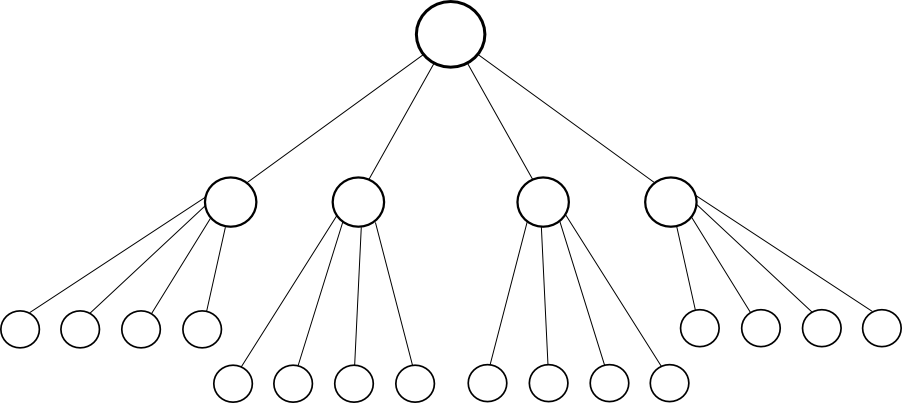
\includegraphics[width=0.5\textwidth]{quad_tree.png}
\end{center}

\begin{itemize}
\item median splitting w/ Surface Area Heuristic \cite{sah} criterion 
\item Quad-tree
  \begin{itemize}
  \item discretizes the geometric primitives and space more finely per level in the tree
  \item makes for more tree nodes to check per query
  \end{itemize}
\item uses SIMD commands to check many nodes at once
\end{itemize}

\end{frame}


\section{Implementation of Embree in DAGMC} % 1-2 slides

\begin{frame}
  \frametitle{DAGMC entities in Embree}

  Embree has a limited capability for representing geometric topology, but enough to construct a mappable representation of DAGMC models.

\begin{center}
  \begin{tikzpicture}

    \node (VolA) [uwstep,text width=2cm] {\small DAGMC Volume};
    \node (SceneA) [embreestep, xshift=-3cm] {\small Embree Scene};

    \node (SurfA)[uwstep,xshift=3.5cm] {\small DAGMC Surface};
    \node (GeomA)[embreestep,xshift=6.5cm] {\small Embree Geometry};
    
    \node (SurfB) [uwstep,xshift=3.5cm,yshift=2cm,label={\small EntityHandle}] {\small DAGMC Surface};
    \node (GeomB) [embreestep,xshift=6.5cm,yshift=2cm,label={\small int id}] {\small Embree Geometry};

    \node (SurfC) [uwstep,xshift=3.5cm,yshift=-2cm] {\small DAGMC Surface};
    \node (GeomC) [embreestep,xshift=6.5cm,yshift=-2cm] {\small Embree Geometry};

    \draw[<->] (VolA) -- (SceneA);
    \draw[<->] (SurfA) -- (GeomA);
    \draw[<->] (SurfB) -- (GeomB);
    \draw[<->] (SurfC) -- (GeomC);
    \draw[->] (VolA) -- (SurfA);
    \draw[->] (VolA) -- (SurfB);
    \draw[->] (VolA) -- (SurfC);
  \end{tikzpicture}
  \end{center}

  
\end{frame}

\begin{frame}
\frametitle{make\_watertight}
\begin{itemize}
\item Applies faceted geometric information from CGM to remove topological ambiguity from the model
\end{itemize}
\includegraphics[scale=0.4, trim = 20 50 0 0]{sealing_ex.png}
\end{frame}




\begin{frame}
  \frametitle{Maintaining watertightness}
  make\_watertight \cite{make_watertight_smith_2010} is an algorithm used to ensure the capability of robust ray tracing

  \begin{center}
    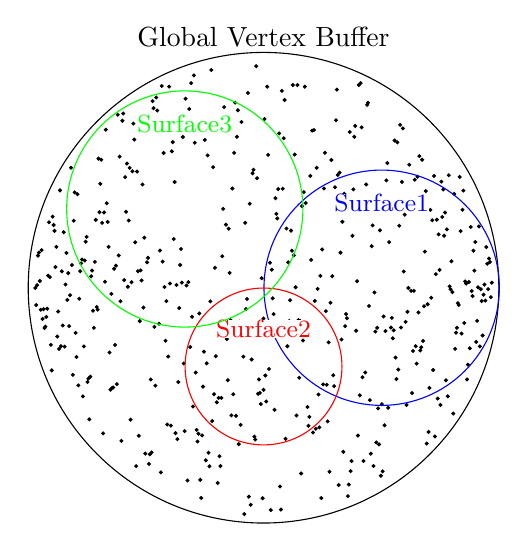
\begin{tikzpicture}
      
    \node[circle,fill=none,minimum width=1cm,text width=6cm,draw=black,label={Global Vertex Buffer}] {};
    \draw plot [only marks, mark=*, mark size=0.5, domain=0:2.9, samples=250] (\x,{rand*sqrt(2.9^2-\x^2)});
    \begin{scope}[yscale=1,xscale=-1]
    \draw plot [only marks, mark=*, mark size=0.5, domain=0:2.9, samples=250] (\x,{rand*sqrt(2.9^2-\x^2)});
    \end{scope}

    \node[circle,outer sep=1pt,fill=none,minimum width=1cm,text width=3cm,draw=blue,xshift=1.5cm] (Surf1Circle) {};
    \node[auto,above=-0.6cm of Surf1Circle,fill=white] (Surf1) {\small \color{blue} Surface1};

    \node[circle,outer sep=1pt,fill=none,minimum width=1cm,text width=2cm,draw=red,yshift=-1cm] (Surf2Circle) {};
    \node[auto,above=-0.7cm of Surf2Circle,fill=white] (Surf2) {\small \color{red} Surface2};

    \node[circle,outer sep=1pt,fill=none,minimum width=3cm,text width=2cm,draw=green,xshift=-1cm,yshift=1cm] (Surf3Circle) {};
    \node[auto,above=-0.6cm of Surf3Circle,fill=white] (Surf3) {\small \color{green} Surface3};
    
    \end{tikzpicture}
  \end{center}
  

\end{frame}

% Maintaining watertightness
   % explain and refer to make_watertight
% Importance of the filter functions
   % allowed compliance with DAGMC conventions
\section{Results} % 2-3 slides

\begin{frame}
\frametitle{Ray Fire Test Models}

An isotropic point source of rays was placed in each of the following models:
\vfill

\begin{tikzpicture}
  \node (sphere) {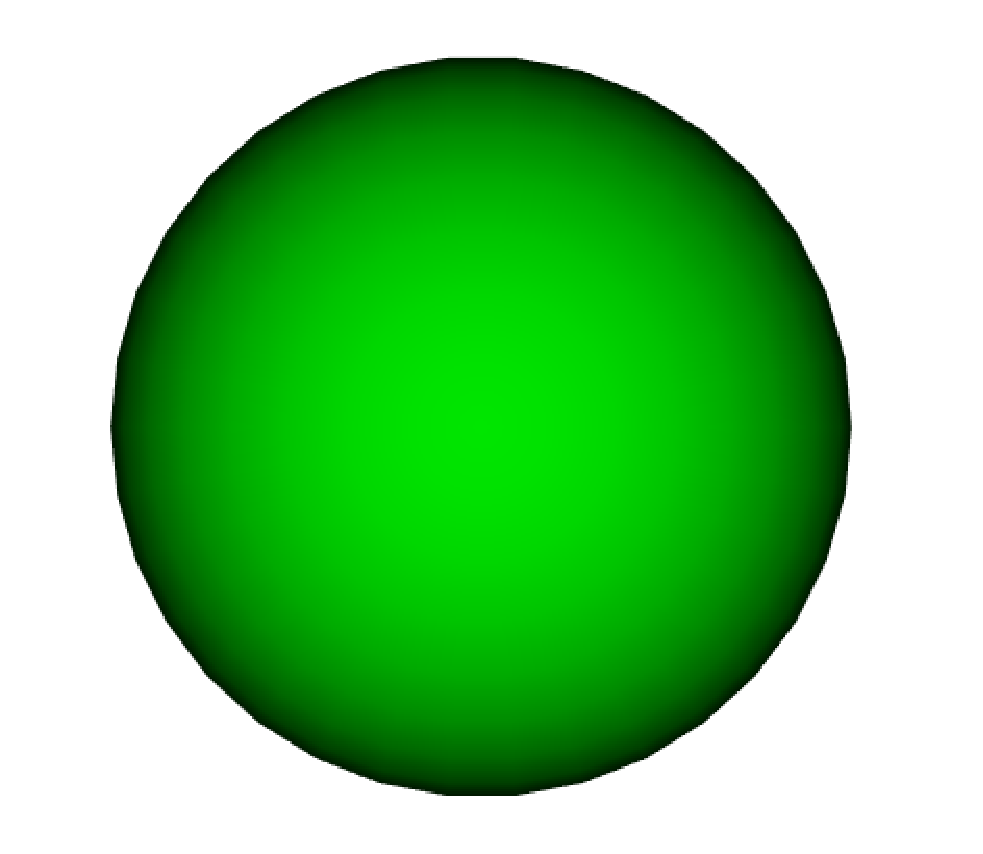
\includegraphics[scale=0.2]{sphere.png}};
  \node (ds) [right =  of sphere] {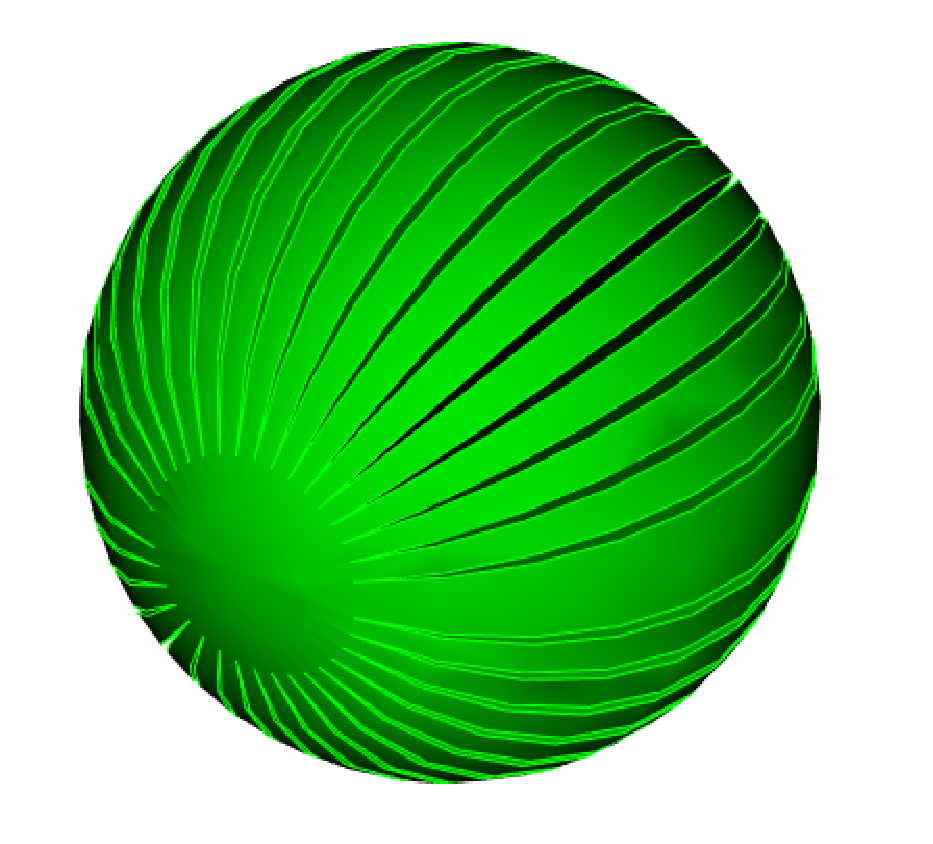
\includegraphics[scale=0.2]{ds.png}};
  \node (larcyl) [right =  of ds] {
\includegraphics[scale=0.2]{larcyl.png}};
  \pause 
  \node (sphere mesh) at (sphere.south east) [rotate=180,xshift=0.5cm] {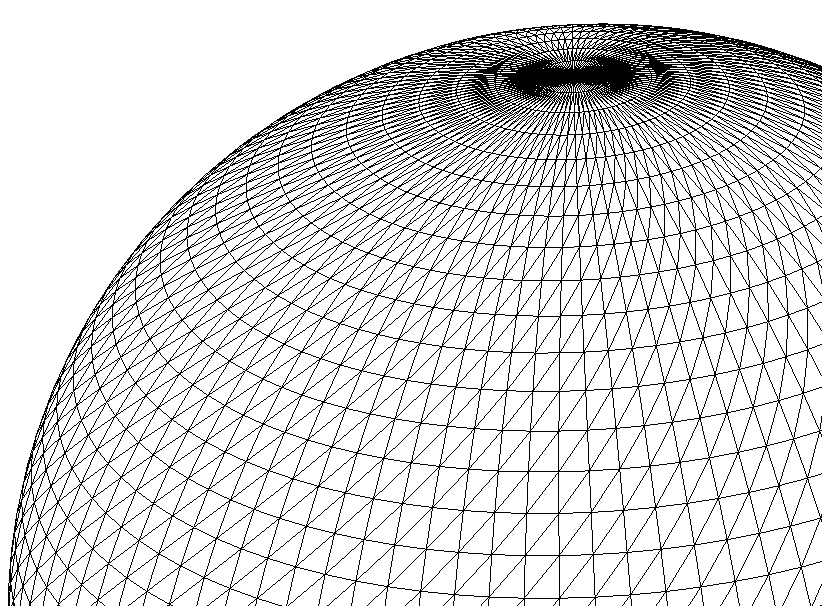
\includegraphics[scale=0.08]{sphere_mesh.png}};
  \pause
  \node (ds mesh) at (ds.north east) {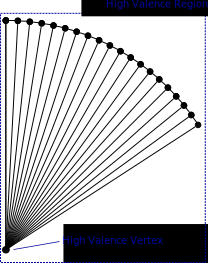
\includegraphics[scale=0.1,xshift=0.5cm]{hv.png}};
  \pause
  \node (lar cyl mesh) at (larcyl.south west) {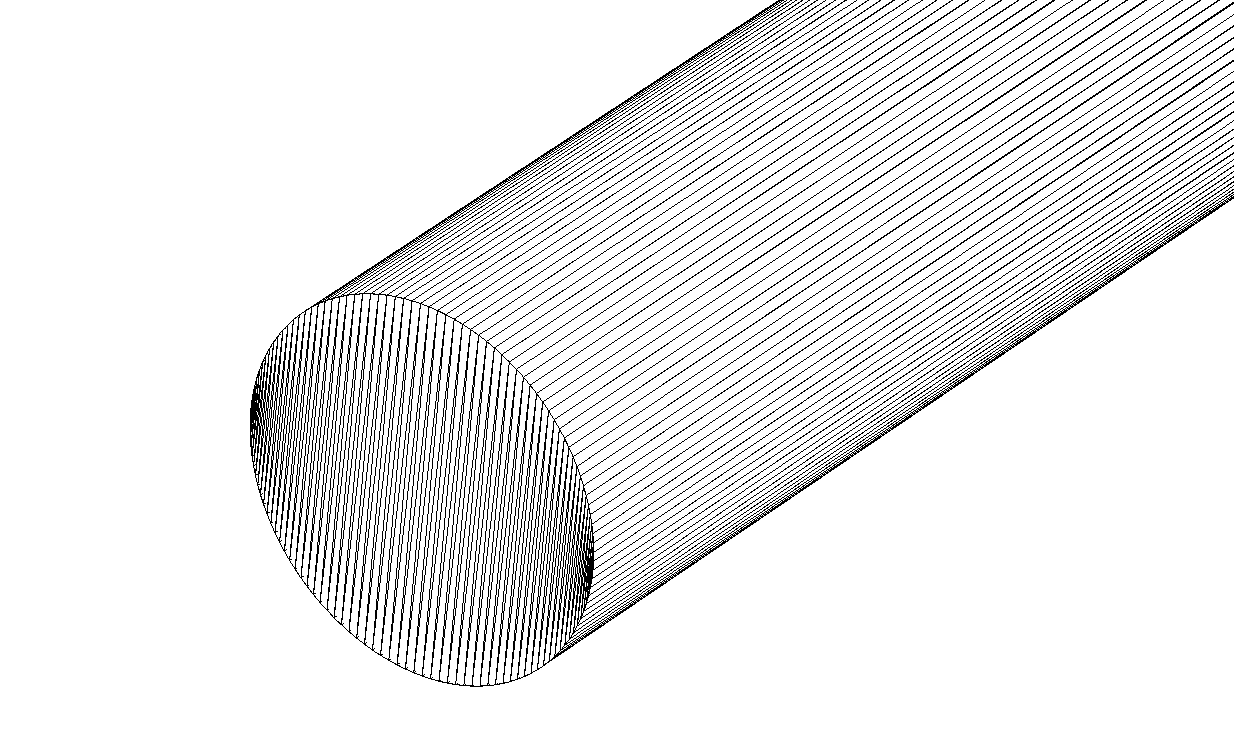
\includegraphics[scale=0.08,crop = 100 0 0 0 ]{lar_cyl_mesh.png}};

\end{tikzpicture}


\end{frame}

\begin{frame}
\frametitle{Ray Fire Timings}
\begin{center}
\begin{columns}
  \column{0.45\textwidth}
  \begin{figure}
    \centering
    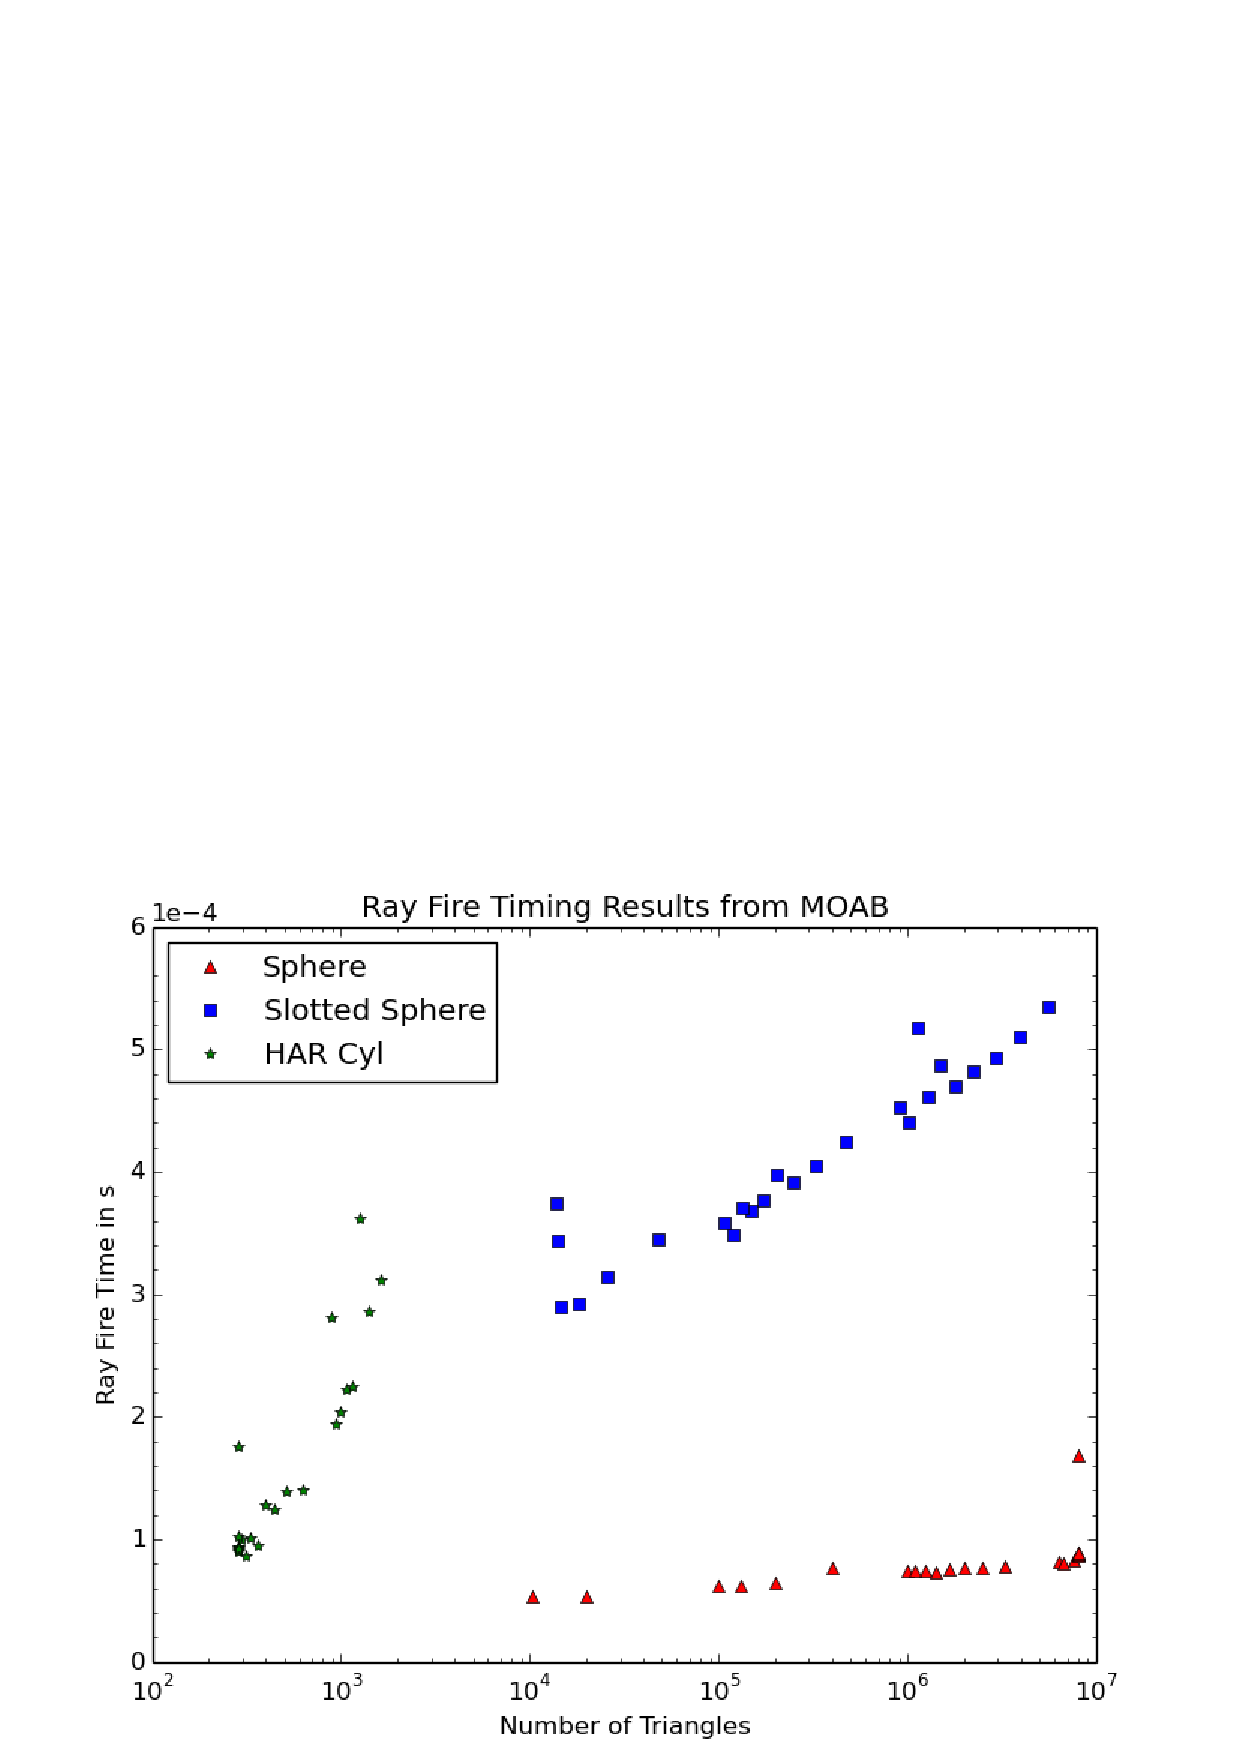
\includegraphics[scale=0.3]{moab_rf.png}
  \end{figure}
  \column{0.45\textwidth}
  \begin{figure}
    \centering
    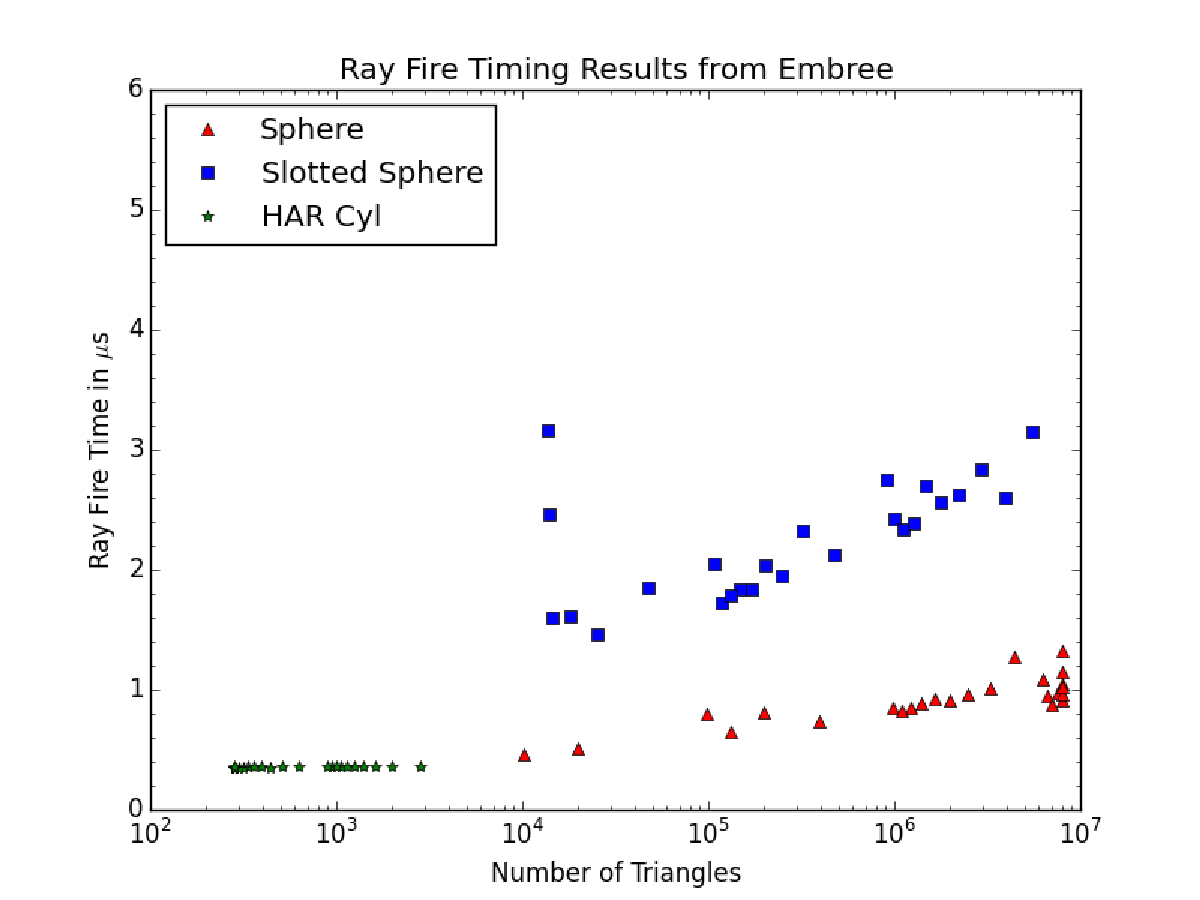
\includegraphics[scale=0.3]{embree_rf.png}
  \end{figure}
\end{columns}
\end{center}
\end{frame}
% Pure ray fire comparison (no transport)
% Single volume tests
% Multiple volume tests
\section{Drawbacks} % 2-3 slides
% Floating precision 
% Robustness needs work, triangle intersector not quite there
% Lost particles in highly complex geometries, most likely due to forced conversion
% back and forth from double to float
% Extra: slide with graphic of our specific problem
\section{Future Work} % 2 slides
% Proof of principle
% Likely to see improvements in our native system using variations of these techniques
% Point them to pyembree for a simple example of a 1-D Monte Carlo calculation in 3 regions


%Citations
\begin{frame}
  \bibliographystyle{ans}
  \bibliography{bibliography}
\end{frame}

%QUESTIONS - 1 slide

\end{document}
